\documentclass{article}
% Primary B — полный вариант статьи
% Shared NeurIPS-RU two-column preamble (input from paper variants).
\usepackage[preprint]{neurips_2025}

\usepackage{fontspec}
\usepackage{polyglossia}
\setdefaultlanguage{russian}
\setotherlanguage{english}
\setmainfont{Liberation Serif}
\setsansfont{Liberation Sans}
\setmonofont{Liberation Mono}

\usepackage{amsmath,amssymb}
\usepackage{booktabs}
\usepackage{multirow}
\usepackage{graphicx}
\usepackage{url}
\usepackage{hyperref}
\usepackage{xcolor}
\usepackage{microtype}
\usepackage{enumitem}

\graphicspath{{images/}{../mmcs-sfedu_thesis7/images/}}

\makeatletter
\renewcommand{\@notice}{%
  \begingroup
    \renewcommand{\thefootnote}{}%
    \footnotetext[0]{\hspace*{-\parindent}\footnotesize\@noticestring}%
  \endgroup
}
\AtBeginDocument{%
  \newgeometry{%
    letterpaper,%
    textheight=9in,%
    textwidth=7in,%
    top=1in,%
    left=0.75in,%
    headheight=12pt,%
    headsep=25pt,%
    footskip=30pt%
  }%
  \setlength{\columnsep}{0.25in}%
  \setlength{\columnseprule}{0pt}%
}
\makeatother

\newcommand{\rem}{\mathrm{REM}}
\newcommand{\elpd}{\mathrm{elpd}}
\newcommand{\PS}{ПС}


\title{Primary~B: размах профиля ПС как единственный признак\\
в байесовской модели разладки (density-safe Beta)}

\author{%
  С.~А.~Пономарёв \\
  Институт математики, механики и компьютерных наук\\
  Южный федеральный университет \\
  \texttt{ponomarev@sfedu.ru} \\
}

\begin{document}

\twocolumn[{%
\maketitle
\begin{abstract}
Фиксируем primary-анализ~\textbf{B}: единственный признак ---
\texttt{daily:range} (\emph{размах профиля ПС}), правдоподобие
\texttt{beta\_constrained} ($\alpha,\beta\ge 1$), не plain Beta.
Отчитываем \emph{всю} confirmatory-тройку разрешений без cherry-pick:
$(N,\mathrm{ov})\in\{(48,0),\,(48,0{,}25),\,(24,0{,}5)\}$ на страте
\texttt{full} ($n{=}33$). Получены
$\mathbb{E}[\tau]\in\{7{,}254;\,7{,}097;\,5{,}747\}$;
нормированный ELPD выше, чем у Primary~A, но при $(24,0{,}5)$ шире
HDI. Plain Beta раздувает ELPD ($\sim\!6{,}64$ vs $\sim\!5{,}19$) ---
артефакт границы~$1$. Вариант~B ближе к классической доктрине
размаха; onset $\tau$ не смешиваем с окном эффекта $2$--$4$\,сут.

\medskip
\noindent\textbf{Ключевые слова:}
размах профиля ПС, beta\_constrained, точка разладки, primary~B,
PSIS-LOO.
\end{abstract}
\vspace{1.0em}
}]

\section{Введение}

Классические нейросейсмоотчёты по площадке ``Институт'' измеряли
\emph{размах профиля ПС} --- $R=\max P-\min P$ по суточному
профилю из $12$ неперекрывающихся $2$-часовых бинов --- и находили
выраженные отклонения в окне примерно $2$--$4$ суток до/после
сильных событий. Июльский байесовский перебор поднял
\texttt{daily:range} с plain~Beta на верх ELPD, но аудит границы
показал: $\sim 25$--$30\%$ значений $R/2$ лежат в $[0{,}9,1]$,
апостериор тянет $\beta\ll 1$, поточечный log-lik коррелирует с
близостью к~$1$ ($r\approx 0{,}8$--$0{,}9$). Это сигнатура
раздувания ELPD, а не однозначный физиологический ранг.

Поэтому primary~\textbf{B} фиксирует \textbf{тот же семантический
признак} (размах), но \textbf{density-safe} likelihood
(\texttt{beta\_constrained}), и требует отчёта по трём разрешениям
сразу --- без выбора ``лучшего'' после просмотра цифр.
Параллельный Primary~A (mean+range) --- отдельная заметка.

Цель модели --- дискретная точка разладки $\tau$ (onset нового
режима на восьми сутках), а не классический контраст ``эффект vs
тихий контроль''.

\section{Данные}

Те же животные, гипнограммы и события, что в Primary~A
\cite{Saevskiy2025,Vyazovskiy2005}: интенсивность $>2$, окно
$8$ суток. Страта primary: \texttt{full} (before +
after\_reversed), $n{=}33$. \textbf{$2024$-$09$-$30$} включён;
неполные after\_reversed с \texttt{exported=False} в LOO не
входят. Влиятельные окна не удаляем ``по Pareto'': на малой
выборке они могут составлять сигнал; with/without --- чувствительность.

\section{Методы}

\subsection{Профиль}

$N$ долей ПС с перекрытием $\mathrm{ov}$; \texttt{rem\_stage}${}=2$.
Классика $(12,0)$ остаётся в таблице чувствительности. Масштаб
пары в $[0,1]$; Beta наблюдает $R/2$.

\subsection{Признак Primary~B}

Только $R=\max_i p_i-\min_i p_i$. Среднее $\bar P$ \emph{не}
входит ($F{=}1$). Это сознательное приближение к классической
метрике размаха профиля ПС.

\subsection{Тройка без cherry-pick}

\begin{center}
\small
\begin{tabular}{llc}
\toprule
$(N,\mathrm{ov})$ & Роль & Связь\\
\midrule
$(48,0)$ & mid/high-$N$, July-подобная & верх ELPD июля\\
$(48,0{,}25)$ & то же $N$, частичный overlap & сглаживание\\
$(24,0{,}5)$ & мост к $(W,S){=}(2,1)$ & рядом с Primary~A\\
\bottomrule
\end{tabular}
\end{center}

\subsection{Модель}

\[
R_t\sim
\begin{cases}
\mathrm{Beta}(\alpha_1,\beta_1)\ \text{на }R_t/2, & t<\tau,\\
\mathrm{Beta}(\alpha_2,\beta_2)\ \text{на }R_t/2, & t\ge\tau,
\end{cases}
\]
с $\alpha_j,\beta_j\ge 1$ (constrained) и
$\tau\sim\mathrm{DiscreteUniform}\{3,\ldots,8\}$, маргинализация,
NUTS/BlackJAX~\cite{HoffmanGelman2014}. Контроли: IIB@$0{,}9$;
diagnostic plain Beta. Скоринг: PSIS-LOO, elpd/$FE'$, LOO-IC
\cite{Vehtari2017}. Бюджет: tune~$500$, draws~$400$, $2$ цепи,
id \texttt{20260806}.

\begin{figure}[t]
  \centering
  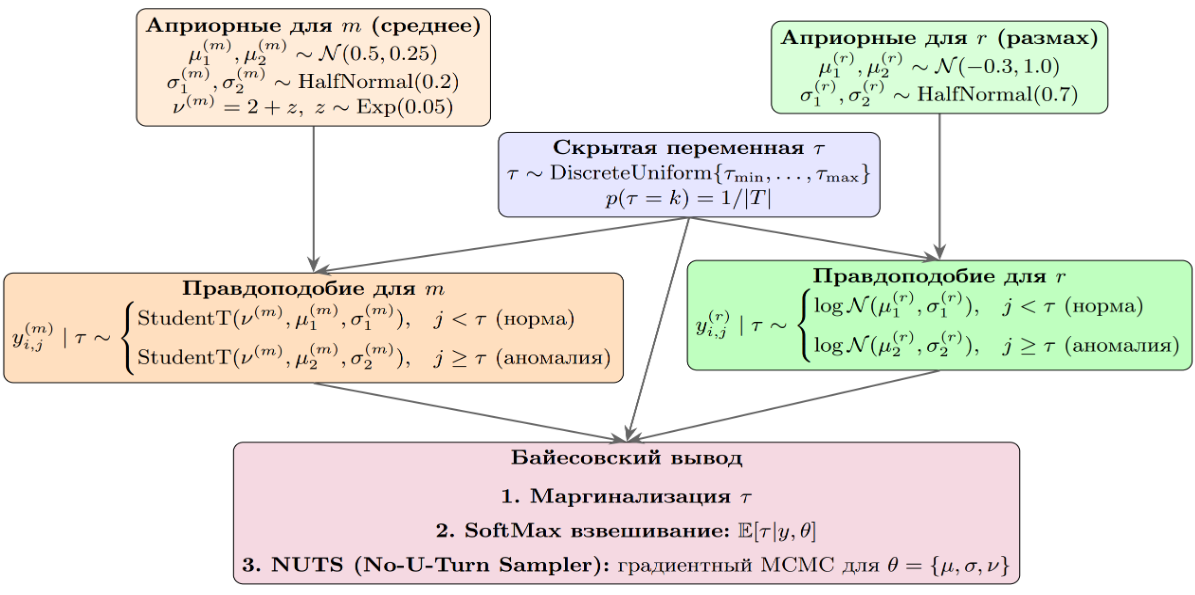
\includegraphics[width=\linewidth]{tau_model.png}
  \caption{Одна разладка на ряде суточных размахов.}
\end{figure}

\section{Результаты тройки}

\begin{table}[t]
\centering
\caption{Primary~B: range + \texttt{beta\_constrained}, full,
$n{=}33$.}
\label{tab:primary-b}
\small
\begin{tabular}{lrrr}
\toprule
$(N,\mathrm{ov})$ & $\mathbb{E}[\tau]$ & HDI$_{60}$ & elpd/$FE'$\\
\midrule
$(48,0)$ & $7{,}254$ & $0{,}258$ & $5{,}187$\\
$(48,0{,}25)$ & $7{,}097$ & $0{,}372$ & $4{,}814$\\
$(24,0{,}5)$ & $5{,}747$ & $2{,}402$ & $4{,}270$\\
\bottomrule
\end{tabular}
\end{table}

При высоком $N$ onset $\approx 7$ суток с узким HDI; при мостовом
$(24,0{,}5)$ --- раньше по среднему, но шире неопределённость.
Заявлять одну точку ``победителем'' нельзя.

\begin{figure}[t]
  \centering
  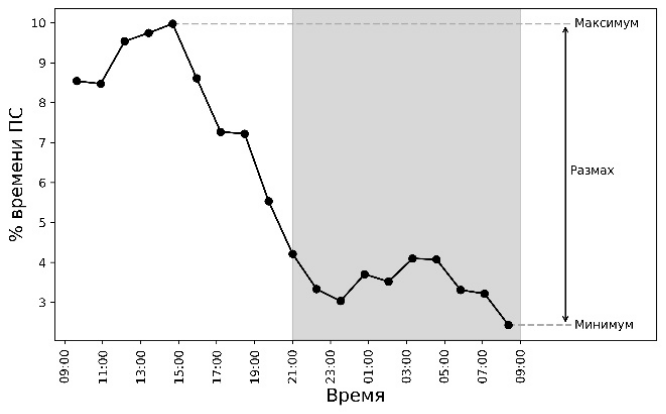
\includegraphics[width=\linewidth]{rem_profile.png}
  \caption{Размах профиля ПС --- разность max и min долей ПС.}
\end{figure}

\section{Почему не plain Beta}

\begin{table}[t]
\centering
\caption{Диагностика границы при $(48,0)$.}
\label{tab:beta-b}
\small
\begin{tabular}{lrr}
\toprule
Likelihood & elpd/$FE'$ & $\mathbb{E}[\tau]$\\
\midrule
plain beta (DIAG) & $6{,}644$ & $6{,}391$\\
\texttt{beta\_constrained} & $5{,}187$ & $7{,}254$\\
IIB@$0{,}9$ & $4{,}843$ & $7{,}016$\\
\bottomrule
\end{tabular}
\end{table}

$\Delta\mathrm{elpd}/FE'\approx 1{,}5$ при том же признаке --- цена
boundary blow-up. $\tau$ остаётся в полосе $\sim 6$--$7{,}5$\,сут:
onset устойчивее LOO-ранга plain Beta. IIB на $(24,0{,}5)$:
$\mathbb{E}[\tau]{=}7{,}646$ с узким HDI у верха prior --- край,
не усреднять.

\begin{figure}[t]
  \centering
  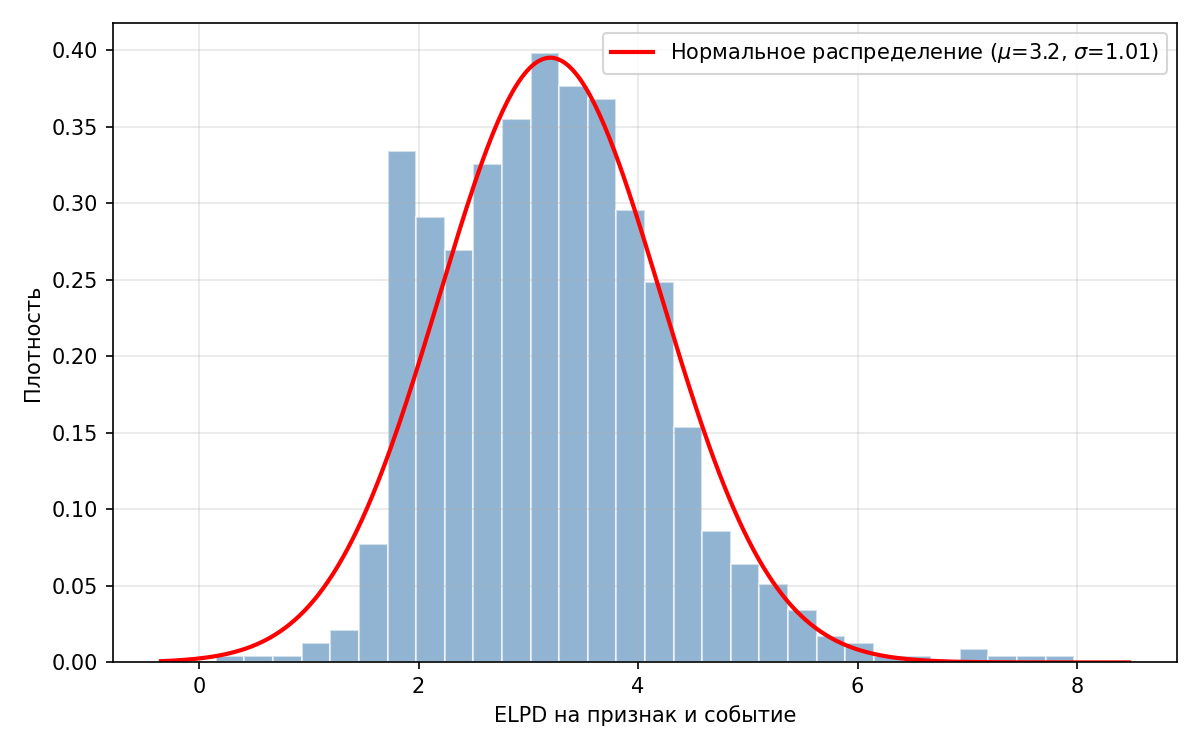
\includegraphics[width=\linewidth]{hist_elpd.png}
  \caption{Большие сетки дают верхний хвост ELPD; для B критичен
  контроль likelihood, а не только хвост.}
\end{figure}

\section{Чувствительность и связь с A}

На таблице feature$\times N$ без plain beta
$\mathbb{E}[\tau]\in[5{,}747;\,7{,}687]$. Range при $(12,0)$:
$\mathbb{E}[\tau]{=}7{,}031$, HDI$_{60}{=}0{,}046$ ---
подозрительно узко. Primary~A (mean+range, $24/0{,}5$):
$\mathbb{E}[\tau]{=}6{,}285$, elpd/$FE'{=}3{,}034$ --- ниже score
($F{=}2$), иной состав признаков. Сравнивать A и B по абсолютному
ELPD можно только qualitatively: у B один признак, у A два.

Негативный контроль \texttt{shuffle\_dates} и drop
$2024$-$09$-$30$ --- в общем integrity-протоколе; заголовок B ---
тройка на full со всеми влиятельными окнами.

\section{Классика $2$--$4$ суток vs $\tau$}

Классика фиксирует, когда размах \emph{велик} относительно тихих
дней. Байесовский $\tau$ --- когда начинается новый режим на
восьмидневном ряде. Оценки совместимы при нарастании эффекта, но
это разные параметры. Primary~B --- современный onset-ответ на
классический вопрос о размахе.

\section{Ограничения}

Малая выборка; одна разладка; artifact-days без маски;
мультисид null ещё не закрыт. Не стресс-биомаркер и не прогноз EQ.

\section{Выводы}

\begin{enumerate}[leftmargin=1.2em,itemsep=0.3em]
  \item Primary~B: \texttt{daily:range}+\texttt{beta\_constrained};
  тройка $(48,0)$, $(48,0{,}25)$, $(24,0{,}5)$.
  \item $\mathbb{E}[\tau]$: $7{,}25$ / $7{,}10$ / $5{,}75$; при
  низком разрешении шире HDI.
  \item Plain Beta завышает ELPD у границы~$1$.
  \item B дополняет A: классический размах vs мост mean+range; оба
  оставляют влиятельные события в выборке.
\end{enumerate}

\begin{ack}
Цифры --- \texttt{integrity\_sensitivity\_full\_seed20260806};
конвейер \texttt{seismic-pipeline}; данные станции ``Институт''.
\end{ack}

{\small
\bibliographystyle{plainnat}
\bibliography{references}
}

\end{document}
